\begin{frame}
\begin{example}
Where is this function discontinuous?
\begin{columns}[c]
\column{.4\textwidth}
\[
f(x) = \lfloor x\rfloor
\]
\ \psset{xunit=1cm, yunit=1cm}
\begin{pspicture}(-1.5, -1.5)(3.8,3.8)
\psframe*[linecolor=white](-1.5,-1.5)(3.8,3.8)
\psaxes[labels=x, ticks=x]{<->}(0,0)(-1.5,-1.5)(3.8,3.8)
\psline(-0.1,1)(0.1,1)
\rput[b](-0.25, 1){$1$}
\psline[linecolor=red](-1,-1)(0,-1)
\fcFullDot{-1}{-1}
\fcHollowDot{0}{-1}

\psline[linecolor=red](0,0)(1,0)
\fcFullDot{0}{0}
\fcHollowDot{1}{0}

\psline[linecolor=red](1,1)(2,1)
\fcFullDot{1}{1}
\fcHollowDot{2}{1}

\psline[linecolor=red](2,2)(3,2)
\fcFullDot{2}{2}
\fcHollowDot{3}{2}

\psline[linecolor=red](3,3)(3.8,3)
\fcFullDot{3}{3}
%\fcHollowDot{4}{3}
\end{pspicture}
%\ 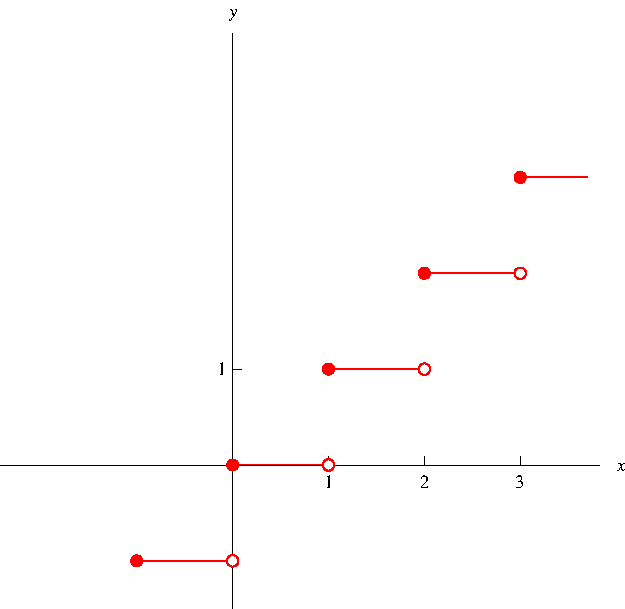
\includegraphics[height=4.5cm]{continuity/pictures/02-05-ex2d.pdf}%
\column{.6\textwidth}
\begin{itemize}
\item<2-| alert@3-4>  $f(1)$ \uncover<4->{exists ($f(1) = 1$).}
\item<2-| alert@5-6>  $\lim\limits_{x\rightarrow 1^+} f(x)$ \uncover<6->{$ = 1$.}
\item<2-| alert@7-8>  $\lim\limits_{x\rightarrow 1^-} f(x)$ \uncover<8->{$ = 0$.}
\item<2-| alert@9-10>  $\lim\limits_{x\rightarrow 1} f(x)$ \uncover<10->{doesn't exist.}
\item<11->  Discontinuous at 1.
\item<12->  Discontinuous at every integer $n$.
\item<13-> The left and right limits both exist but are not equal. 
\item<14-> Such discontinuities are called jump discontinuities (the function appears to ``jump'').
\end{itemize}
\end{columns}
\end{example}
\end{frame}